% =============================================================================
% SAMBP: Confidence Gating Decision Tree
% File: confidence_gating_decision.tex
% Description: Flowchart for confidence-based decision arbitration
% =============================================================================

\documentclass[tikz,border=10pt]{standalone}
\usepackage{tikz}
\usepackage{amsmath}
\usetikzlibrary{shapes,shapes.geometric,arrows,arrows.meta,calc,positioning,fit,decorations.pathmorphing}

\begin{document}

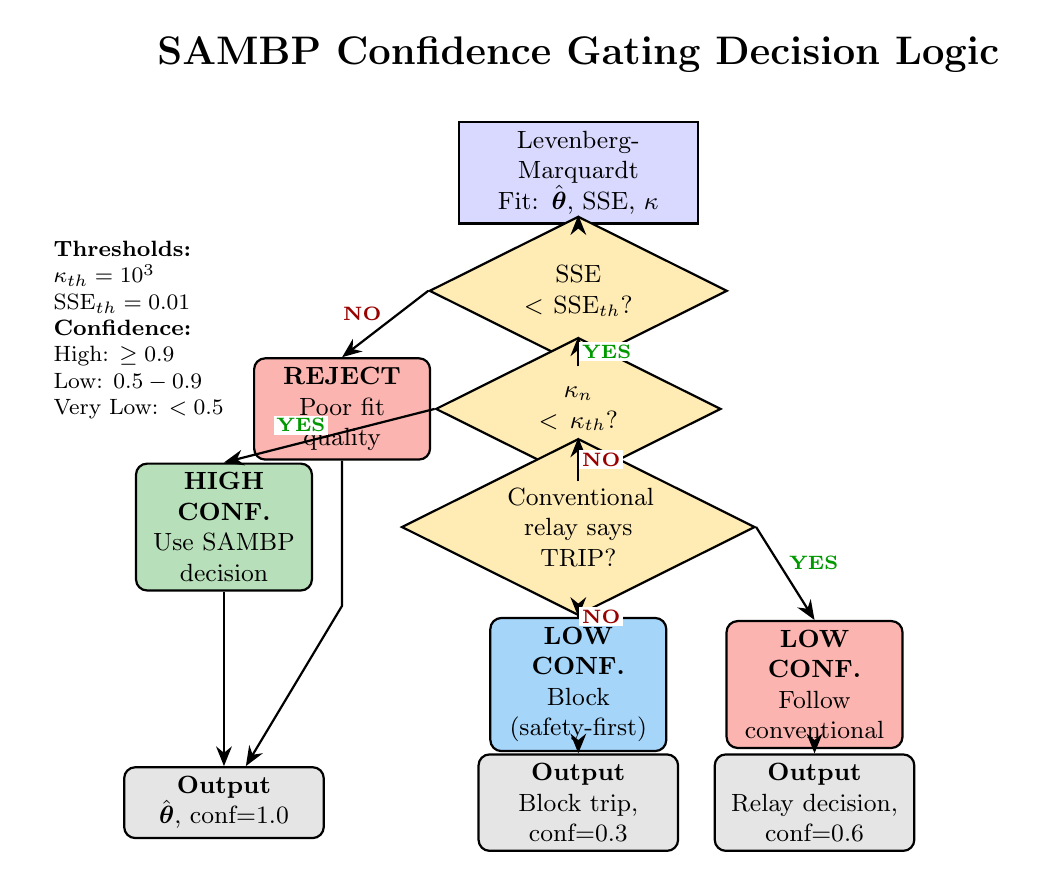
\begin{tikzpicture}[
    node distance=1.2cm,
    font=\small,
    >=latex,
]

\definecolor{decisionColor}{RGB}{255, 193, 7}
\definecolor{highConfColor}{RGB}{76, 175, 80}
\definecolor{lowConfColor}{RGB}{244, 67, 54}
\definecolor{neutralColor}{RGB}{33, 150, 243}

\tikzset{
    decision/.style = {diamond, aspect=2, minimum width=2.2cm, minimum height=0.9cm,
                       text centered, text width=1.8cm, draw=black, thick, fill=decisionColor!30},
    high_conf/.style = {rectangle, rounded corners, minimum width=2.2cm, minimum height=0.7cm,
                        text centered, text width=2cm, draw=black, thick, fill=highConfColor!40},
    low_conf/.style = {rectangle, rounded corners, minimum width=2.2cm, minimum height=0.7cm,
                       text centered, text width=2cm, draw=black, thick, fill=lowConfColor!40},
    neutral/.style = {rectangle, rounded corners, minimum width=2.2cm, minimum height=0.7cm,
                      text centered, text width=2cm, draw=black, thick, fill=neutralColor!40},
    arrow/.style = {thick, -{Stealth[length=2.5mm, width=2mm]}},
    yes_label/.style = {font=\scriptsize\bfseries, color=green!60!black, fill=white, inner sep=1pt},
    no_label/.style = {font=\scriptsize\bfseries, color=red!60!black, fill=white, inner sep=1pt}
}

% Title
\node at (7.5, 11) {\Large \textbf{SAMBP Confidence Gating Decision Logic}};

% =========== PARAMETER ESTIMATION ===========
\node[rectangle, minimum width=3cm, minimum height=0.8cm, text centered,
      text width=2.8cm, draw=black, thick, fill=blue!15] (lm_fit) at (7.5, 9.5) {
    Levenberg-Marquardt Fit: $\hat{\boldsymbol{\theta}}$, $\text{SSE}$, $\kappa$
};

% =========== DECISION TREE ===========

% Level 1: SSE threshold
\node[decision] (sse_check) at (7.5, 8) {$\text{SSE}$\\ $< \text{SSE}_{th}$?};
\draw[arrow] (lm_fit) -- (sse_check);

% SSE NO path - reject
\node[low_conf] (sse_reject) at (4.5, 6.5) {\textbf{REJECT}\\Poor fit quality};
\draw[arrow] (sse_check.west) -- (sse_reject.north)
    node[no_label, midway, above left] {NO};

% SSE YES path - continue to kappa check
\draw[arrow] (sse_check.south) -- ++(0,-0.5);

% Level 2: Condition number
\node[decision] (kappa_check) at (7.5, 6.5) {$\kappa_n$\\ $< \kappa_{th}$?};
\draw[arrow] (sse_check.south) -- (kappa_check)
    node[yes_label, midway, right] {YES};

% Kappa HIGH path
\node[high_conf] (kappa_high) at (3, 5) {\textbf{HIGH CONF.}\\Use SAMBP decision};
\draw[arrow] (kappa_check.west) -- (kappa_high.north)
    node[yes_label, midway, above left] {YES};

% Kappa LOW path - check conventional relay
\draw[arrow] (kappa_check.south) -- ++(0,-0.5);
\node[decision] (conv_check) at (7.5, 5) {Conventional\\relay says\\TRIP?};
\draw[arrow] (kappa_check.south) -- (conv_check)
    node[no_label, midway, right] {NO};

% Conventional YES - TRIP
\node[low_conf] (conv_trip) at (10.5, 3) {\textbf{LOW CONF.}\\Follow conventional};
\draw[arrow] (conv_check.east) -- (conv_trip.north)
    node[yes_label, midway, above right] {YES};

% Conventional NO - BLOCK
\node[neutral] (conv_block) at (7.5, 3) {\textbf{LOW CONF.}\\Block (safety-first)};
\draw[arrow] (conv_check.south) -- (conv_block)
    node[no_label, midway, right] {NO};

% Final outputs
\node[rectangle, rounded corners, minimum width=2.5cm, minimum height=0.8cm,
      text centered, text width=2.3cm, draw=black, thick, fill=black!10] (output1) at (3, 1.5) {
    \textbf{Output}\\$\hat{\boldsymbol{\theta}}$, conf=1.0
};
\node[rectangle, rounded corners, minimum width=2.5cm, minimum height=0.8cm,
      text centered, text width=2.3cm, draw=black, thick, fill=black!10] (output2) at (10.5, 1.5) {
    \textbf{Output}\\Relay decision, conf=0.6
};
\node[rectangle, rounded corners, minimum width=2.5cm, minimum height=0.8cm,
      text centered, text width=2.3cm, draw=black, thick, fill=black!10] (output3) at (7.5, 1.5) {
    \textbf{Output}\\Block trip, conf=0.3
};

\draw[arrow] (kappa_high) -- (output1);
\draw[arrow] (conv_trip) -- (output2);
\draw[arrow] (conv_block) -- (output3);
\draw[arrow] (sse_reject) -- ++(0,-2.5) -- (output1);

% Annotations
\node[font=\footnotesize, anchor=west] at (0.5, 7.5) {
    \begin{tabular}{l}
    \textbf{Thresholds:} \\
    $\kappa_{th} = 10^3$ \\
    $\text{SSE}_{th} = 0.01$ \\
    \textbf{Confidence:} \\
    High: $\geq 0.9$ \\
    Low: $0.5-0.9$ \\
    Very Low: $< 0.5$
    \end{tabular}
};

\end{tikzpicture}

\end{document}
